\documentclass[pdflatex,lineno,sn-nature]{sn-jnl}
\usepackage{graphicx,booktabs,array,amsmath,amssymb,xurl,placeins}
\geometry{reset,a4paper,twoside,bindingoffset=6mm,margin=23mm}
\hypersetup{bookmarksdepth=2}
\emergencystretch=2em
\raggedbottom
\setlength{\bibsep}{0pt}
\newcommand{\PopTwenty}{1.665}
\newcommand{\BuiltTwenty}{197.5}
\newcommand{\PopPctTwenty}{7.40}
\newcommand{\PopThirty}{3.020}
\newcommand{\BuiltThirty}{325.6}
\newcommand{\PopPctThirty}{13.42}
\newcommand{\PopForty}{4.891}
\newcommand{\BuiltForty}{464.6}
\newcommand{\PopPctForty}{21.74}
\newcommand{\PopTotal}{22.501}
\newcommand{\BuiltTotal}{1253.6}
\newcommand{\UniformOneMin}{4.763}
\newcommand{\UniformBiasMin}{57.7}
\newcommand{\UniformOneMax}{4.770}
\newcommand{\UniformBiasMax}{57.9}
\newcommand{\GHSLJointPct}{13.37}
\newcommand{\GHSLJointCommon}{2.989}
\newcommand{\WPJointPct}{23.20}
\newcommand{\WPJointCommon}{5.186}
\newcommand{\EpochOldPct}{20.86}
\newcommand{\EpochOldCommon}{4.664}
\newcommand{\EpochNewPct}{20.28}
\newcommand{\EpochNewCommon}{4.534}
\newcommand{\JointExcluded}{142.9}
\newcommand{\SampleTwentyEight}{3.051}
\newcommand{\SampleFiftySix}{3.232}
\newcommand{\SampleOneTwelve}{3.369}
\newcommand{\SampleTwoTwentyFour}{3.301}
\newcommand{\DWRTotal}{598098}
\newcommand{\DWRUnsupported}{1710}
\newcommand{\DWRSupportPct}{99.71}
\newcommand{\DWRUniformMin}{9022}
\newcommand{\DWRUniformMax}{9556}

\newcommand{\InteriorPopulationMin}{99.27}
\newcommand{\InteriorPopulationMax}{99.49}
\newcommand{\InteriorBiasMin}{58.24}
\newcommand{\InteriorBiasMax}{58.56}
\newcommand{\InteriorErrorMin}{98.55}
\newcommand{\InteriorErrorMax}{98.87}

\newcommand{\CrossGHLow}{51.3}
\newcommand{\CrossGHHigh}{55.6}
\newcommand{\CrossWPLow}{8.6}
\newcommand{\CrossWPHigh}{9.1}

\begin{document}
\title[Spatial aggregation and InSAR support]{Spatial aggregation alters population-weighted estimates of InSAR observation support}
\author[1]{\fnm{Zixuan} \sur{Liu}}
\author*[2,3]{\fnm{Wei} \sur{Xiong}}\email{xw@mail.hbut.edu.cn}
\affil[1]{\orgname{Detroit Green Technology Institute, Hubei University of Technology}, \orgaddress{\city{Wuhan}, \postcode{430068}, \country{China}}}
\affil[2]{\orgname{School of Electrical and Electronic Engineering, Hubei University of Technology}, \orgaddress{\city{Wuhan}, \postcode{430068}, \country{China}}}
\affil[3]{\orgname{Department of Computer Science and Engineering, University of South Carolina}, \orgaddress{\city{Columbia}, \postcode{29201}, \state{SC}, \country{USA}}}
\abstract{Population-weighted assessments of interferometric synthetic aperture radar (InSAR) observation support depend on how population is allocated within reporting units. Spatial aggregation can change these assessments even when the observations are unchanged. We isolate this effect by comparing allocation rules under a fixed geographic domain, support field and population total. In the Chao Phraya footprint, uniform allocation within 1-km cells increases the mean support deficit by 57.7--57.9\% relative to native population-model allocation, equivalent to 7.75--7.78 percentage points of the domain total. Within-cell covariance between population and support explains this difference, which persists after excluding boundary cells. Crossed population-model and interferogram-sampling comparisons preserve its direction but change its magnitude. Shifts as a share of total population are smaller for the final processing mask and in the California cases. Controlled missingness shows that small errors where estimates remain available can coexist with substantial unestimated population allocation. The primary deficit averages unsupported model allocation over area and interferogram pairs; it does not identify subsidence exposure. Population-weighted reporting should therefore preserve the spatial association between population and observation support and report sensitivity to allocation and sampling.}
\keywords{InSAR, population allocation, observation support, coherence, spatial scale, reproducibility}
\maketitle
% The sn-jnl class globally disables top floats while formatting the title.
% Restore ordinary in-text float placement after the title page is complete.
\makeatletter\global\@topnum=5\makeatother
\raggedright

\section{Introduction}
Population-based assessments of land subsidence combine information on ground deformation with the spatial distribution of people. Interferometric synthetic aperture radar (InSAR) applications now include urban population shares above subsidence-rate thresholds \citep{ao2024national}, nationwide exposure inventories, building-level diagnostics and population-weighted assessments of coastal relative sea-level rise \citep{xiong2026nationwide,yang2026buildingrisk,oelsmann2026coastal}. Interpreting these summaries requires specifying both where observations provide support and how population is assigned within reporting units. Identical observations can yield different population-weighted summaries when population is redistributed within those units.

Spatially selective measurement is an established concern in InSAR. Persistent-scatterer, small-baseline and distributed-scatterer methods address this selectivity \citep{ferretti2001ps,berardino2002sbas,ferretti2011squeeSAR}, while LiCSBAS and MintPy provide diagnostics for unwrapped coverage, coherence, temporal connectivity, residuals and uncertainty \citep{morishita2020licsbas,yunjun2019mintpy}. Published assessments also combine quality screening with geodetic comparisons. The Mexico-wide assessment applied temporal-coherence screening and compared InSAR estimates with GPS observations \citep{fernandeztorres2024mexico}, and Ohenhen et al. evaluated rates against 154 GNSS stations across 28 US cities \citep{ohenhen2025uscities}. Published Bangkok studies provide further leveling and CORS comparisons, with their spatial, temporal and station-specific qualifications detailed in Supplementary S3 \citep{luachapichatikul2020bangkok,pumpuang2024bangkapi,aieorattanawadee2022bangkok}. Murray et al. also noted that motion between buildings may remain undetected and require additional observations \citep{murray2025hawaii}. These practices and stated limitations provide an essential basis for interpreting displacement measurements and their spatial support.

Population allocation introduces a further step when displacement products are combined with demographic data. Blackwell et al. combined multiple radar datasets with GNSS and estimated community exposure assuming a uniform population distribution within each community \citep{blackwell2020california}. Ohenhen et al. assigned census-block population to subsidence classes using each block's median InSAR-pixel rate \citep{ohenhen2025uscities}. These explicit choices concern different reporting units and target quantities. Here, we focus on allocation under a specified observation-support field. Holding the geographic domain, support field and population total fixed allows the contribution of allocation to be measured separately from changes in the observations.

Areal interpolation and dasymetric mapping provide established approaches to allocating population within coarse units \citep{eicher2001dasymetric,mennis2003population}. A finer population grid preserves more of the selected model's spatial structure, but does not establish household-level accuracy. The issue examined here is whether aggregation retains the spatial association between population and observation support. Replacing the average of their product with the product of their separate averages omits the within-unit covariance. This relationship explains how aggregation can change a population-weighted summary even when observations remain unchanged. The direction and practical magnitude of the effect depend on the inputs and require evaluation for the population models and support definitions being used.

Here, we quantify this aggregation effect in the Chao Phraya study footprint, with additional comparisons in California. We relate differences between allocation rules to within-cell covariance and assess sensitivity to population models, grid design and interferogram sampling. Controlled missingness tests distinguish errors at retained locations from population allocation left unestimated, while comparisons across processing stages assess dependence on the definition of support. The resulting quantities describe population-weighted observation support and do not directly estimate subsidence exposure. Together, these analyses quantify the magnitude and limits of aggregation effects and provide a reporting procedure that preserves the spatial association between population and support.

\section{Materials and methods}
\subsection{Geographic domain, support field and population allocation}
We distinguish three objects: the geographic domain $D$ (area of interest, AOI), a support field $s(x)\in[0,1]$, and a nonnegative exposure density $\rho(x)$. Our primary Chao Phraya domain is the native Global Human Settlement Layer (GHSL) pixels whose centers lie in the frozen finite footprint of 18,077 archived VLM cells. It includes 1,807,700 GHSL 3-arc-second pixels and does not condition on a velocity threshold. This explicit pixel-defined boundary is held fixed in all primary allocation experiments. Because its footprint is inherited from finite source-product cells, this design does not assess locations outside that original footprint or establish complete coverage of the geographical delta.

The archived VLM GeoTIFF matches the Chao Phraya file in the global-delta dataset accompanying Ohenhen et al. \citep{ohenhen2026deltas,ohenhen2025deltadata}. That study used WabInSAR. Our LiCSAR quality sample is a different processing chain and cannot be interpreted as the validity mask of the WabInSAR product. Moreover, the public GeoTIFF lacks an explicit stored-unit tag establishing the archived factor-of-ten conversion. We therefore retain the inherited strong-deformation selection only as a clearly labeled supplementary sensitivity. Neither that conversion nor a cross-product quality proxy determines the primary geographic population denominator.

For pair $j$, let $M_j(x)$ be one when unwrapped phase is finite, passes its raster validity mask and is nonzero, and, for the joint screens, the associated byte coherence divided by 255 is at least $q$. The unwrapped zero rule is product-specific \citep{licsarproducts}. We evaluate $q=0.2,0.3,0.4$ and unwrapped validity alone. Source-grid boundaries and the actual GDAL affine transforms, including point registration, are used independently for coherence and unwrapped products. We split at both sets of boundaries, intersect the binary masks first, and then integrate. Multiplying separately averaged fractional masks would not give their spatial intersection.

For GHSL pixel $p$ with area $A_p$, the reported support is
\begin{equation}
s_p=\frac{1}{N A_p}\sum_{j=1}^{N}\int_p M_j(x)\,\mathrm{d}A.
\label{eq:support}
\end{equation}
Thus $s_p$ is mean area--pair support at the exposure grid. It is distinct from the area whose individual locations pass a fixed number of pairs, from a binary majority classification at a cell center, and from final inversion validity. We assume each GHSL pixel's population or built-surface total is uniform within that pixel when integrating its intersections. Spherical rectangular areas use longitude and sine-latitude boundaries.

\subsection{Continuous support summaries and their interpretation}
With nonnegative allocated exposure $E_p$, define supported allocation $S_E=\sum_p E_p s_p$, mean support deficit $U_E=\sum_p E_p(1-s_p)$, and total $T_E=\sum_p E_p$. By construction, $S_E+U_E=T_E$. Population-valued $U_E$ is an average unsupported allocation over the selected pairs. For example, a pixel assigned 100 people and mean support 0.8 contributes 20 population-allocation units to $U_E$. Those units express a weighted average over area and pairs; they do not identify 20 particular residents. As an allocation example, two equal-area fine pixels with populations 90 and 10 and supports 1 and 0 have a native deficit of 10. Spreading the same total uniformly across their combined area gives 50. Reversing the support pattern gives a native deficit of 90 and the same uniform estimate of 50. The sign of the allocation difference depends on the spatial association between population and support. $U_E$ does not count unique residents who lacked observations throughout the study period. Neither population-valued nor built-surface-valued $U_E$ identifies confirmed deformation, vulnerability, loss or damage.

The weighted support distribution is
\begin{equation}
F_E(t)=\frac{\sum_p E_p\,\mathbf{1}(s_p<t)}{T_E},\qquad
\int_0^1 F_E(t)\,\mathrm{d}t=\frac{U_E}{T_E}.
\end{equation}
We show the full distribution rather than selecting a single majority cutoff. The integral identity concerns the empirical step distribution; its exact numerical check uses the sorted support values, not a trapezoidal approximation to the 101-point display curve.

\subsection{Matched-target allocation and grid experiments}
The center, area-weighted and ancillary-weighted rules represent distinct choices within established areal-interpolation practice \citep{eicher2001dasymetric,mennis2003population}. Supplementary S6 states their information requirements and which comparisons are actually performed. Native GHSL allocation is the common model reference for these tests; comparisons with deformation imputation or multi-sensor retrieval would require a different target and additional observations.

We conservatively transfer extensive first and cross moments to a 50-m UTM integration grid (zone 47N), then repartition them into 250-, 500-, 1,000- and 2,000-m cells. Each size has four origins formed by zero and half-cell shifts in each axis. Included-domain area is retained in partial boundary cells; population is not extrapolated into the omitted area. The 50-m reprojection preserves the input totals within the stated numerical tolerance. A separately recomputed 25-m integration diagnoses approximation sensitivity, including its measured small reprojection drift (Supplementary Information).

Within cell $c$, let $P_c=\int_c\rho\,\mathrm{d}A$, $H_c=\int_c\rho s\,\mathrm{d}A$, $A_c=\int_c\mathrm{d}A$ and $Q_c=\int_c s\,\mathrm{d}A$. Native-model reference deficit is $P_c-H_c$, while uniform allocation gives $P_c(1-Q_c/A_c)$. Their difference is
\begin{equation}
U_{\rm uniform}-U_{\rm native}
=\sum_c\left(H_c-\frac{P_c Q_c}{A_c}\right)
=\sum_c A_c\operatorname{Cov}_{A,c}(\rho,s).
\label{eq:covariance}
\end{equation}
Preserving $H_c$ avoids replacing the native reference with the product of separately averaged population and support fields. The center method applies support from the fine pixel containing each coarse center; centers outside the fixed domain receive zero support. We report signed aggregate allocation discrepancies, discrepancies normalized by the fixed AOI total, and cell-level absolute discrepancies. The native GHSL reference is a controlled allocation model, not observed household truth. To separate interior allocation effects from boundary handling, we additionally repeat the primary comparison on coarse rectangles wholly contained in the pixel-defined domain. The domain boundary is formed from the native GHSL mask, densified at native-pixel spacing and transformed to UTM before the containment test. Interior and boundary subsets retain their own population and reference-deficit denominators; full-domain results remain the primary comparison.

\subsection{Artificial masking with known reference quantities}
A fixed Bangkok rectangle (100.35--100.75$^\circ$ E, 13.55--13.95$^\circ$ N) supplies the population and built-surface fields for controlled masking. This rectangular experiment is separate from the VLM-footprint domain. We remove 10\%, 30\% or 50\% of fine pixels using random scores, spatially smoothed random scores, and scores positively or negatively associated with log population density. We fix the seed and run 100 repetitions per combination. We report all 100 realizations for each missingness mechanism and removal fraction.

Methods use identical introduced masks and coarse-cell population totals. We compare uniform-area allocation, center sampling and allocation proportional to fine built area, with an area fallback where built area is zero. Grids contain 5, 10 or 20 native pixels with two origins; these angular grids are not described as exact metric cells. We evaluate against the known removed allocation $U_{\rm ref}$. Percentile ranges describe variation over the introduced masks, conditional on the fixed models. They are not confidence intervals for real population or InSAR accuracy. Built weighting is not independent validation because GHSL population already uses built-environment information.

We also construct three explicit synthetic hazard fields: positive density association, negative association and an independent spatial field. Rates are assigned either $-10$ or $0$ mm yr$^{-1}$ solely to define known threshold membership. For observed threshold allocation $T_{\rm obs}$ and unknown allocation $U$, the nonparametric identification interval is $[T_{\rm obs},T_{\rm obs}+U]$. Checking that synthetic truth lies inside this interval verifies the accounting bound; it does not validate a physical prediction or establish 95\% coverage.

\subsection{Sampling, population products and land cover}
The legacy sample has 28 pairs from 2016--2022. We evaluate year omissions, start-date quarters and temporal-baseline groups. A larger pool contains eight pairs per year--quarter stratum, totaling 224. Selection uses dates and short/long baseline classes before expanded support outcomes are computed. Before outcome extraction, adjacent ranks in even quarters were swapped to improve balance in the smallest nested sample; both rank plans and the amendment are preserved. Available baseline composition is reported explicitly. Nested ranks produce 28, 56, 112 and 224 pairs. An additional 100 draws without replacement per sample size characterize sampling variation within this fixed pool. They do not account for unknown interferograms outside the pool, nor estimate independent-observation confidence bounds.

We compare GHSL R2023A epoch-2020 population at 3 arcsec with WorldPop's Thailand 2020 unconstrained UN-adjusted population-count product at 3 arcsec \citep{pesaresi2024ghsl,worldpop2020}. Source counts are transferred by spherical source-area fractions, not by interpolation of density values as if they were counts. Native totals, jointly valid coverage and common-total normalized results are all reported. GHSL 2015/2020 epoch comparisons hold resolution at 30 arcsec. Neither population product is local census truth, and epoch differences combine demographic and model effects.

\paragraph{Crossed aggregation sensitivity.} To test the aggregation effect directly across inputs, we cross GHSL and WorldPop 2020 allocations with the legacy 28-pair and expanded 224-pair support fields at $q=0.3$. All four combinations use the same two-model common-valid domain and the same total population, set to the GHSL total on that domain. The domain is fixed before comparing aggregation outputs. Each combination compares native-model and uniform allocation within 1-km cells at four origins, using conserved area, supported area, population and population--support cross moments. We report differences relative to the native-model deficit and to the common total. A 25-m integration diagnostic checks the production 50-m transfer. Pair selection and composition change with pair number; the experiment does not isolate sample size alone. Supplementary S18 retains all 16 model--sample--origin cases.

ESA WorldCover 2021 v200 provides native 10-m land classes \citep{worldcover2021}. We calculate their fractional areas inside each GHSL pixel and allocate that pixel's population uniformly across those fractions. Allocation to tree-covered fractions follows the within-pixel uniformity assumption and does not identify residential locations. The 2021 land-cover epoch also differs from the population epoch and the multi-year radar sample.

\subsection{Matched processing and a second published-support case}
We define a separate Bangkok urban--periurban rectangle (100.35--100.65$^\circ$ E, 13.65--14.05$^\circ$ N) before examining processing outcomes. All 437 catalogue pairs with both dates in 2019--2020 and temporal baseline at most 96 days are retrieved and checked. This date graph contains 104 acquisitions and is connected. Native unwrapped phase and byte coherence are aligned by nearest sampling, using each source's actual GDAL transform, onto the first unwrapped raster's approximately $0.001^\circ$ grid. LiCSBAS2 steps 11--16 provide quality rejection, loop closure, small-baseline inversion, velocity spread, multi-index masking and filtering \citep{morishita2020licsbas,licsbas2}. We retain upstream scientific routines and fixed C-band defaults; automatic relaxation of masking thresholds is disabled. Supplementary S17 records the exact version and parameters.

Before reading pixel quality, 44 pair edges are randomly selected for holdout while preserving global acquisition-date connectivity. The other 393 pairs are processed separately through the same workflow. Held-out phase differences are converted to relative line-of-sight (LOS) displacement and referenced to the training solution's reference pixel. Predicted differences come from the unfiltered training cumulative displacements at those two dates. On observations evaluable by all methods, we also compare predictions from the training linear velocity and from zero relative displacement. Missing training dates or invalid held-out phase at the training reference are recorded as exclusions. Predictive strata use training-pair support and the training mask, excluding held-out coherence from their definition. All held-out dates remain represented in training; this tests edge reconstruction rather than forecasting new acquisition dates. Pairs share acquisitions and date-dependent atmospheric phase, so we report descriptive residuals without an independent-replicate confidence interval. No GNSS calibration, vertical decomposition or recovery of permanently absent observations is claimed.

We separately compare legacy 28-pair support and matched-stack support with the full-stack quality mask, reporting pixel- and population-weighted confusion counts, support-bin validity, velocity spread and inversion residuals. Native GHSL counts are transferred by source-area fractions to the processing grid. Mask association is partly built into the algorithm because coherence contributes to its quality criteria; the edge holdout adds a distinct internal predictive check. The legacy comparison additionally differs in acquisition period (2016--2022 versus 2019--2020); the matched input diagnostic provides a within-period comparison. This experiment evaluates a specified LiCSAR/LiCSBAS chain and does not test the validity of the WabInSAR source raster.


For the independent geometry case, we select a fixed Fresno rectangle (119.9--119.7$^\circ$ W, 36.6--36.85$^\circ$ N) before inspecting its support results. The California Department of Water Resources (DWR) 2026Q1 service supplies actual polygons representing its 100-m measurement cells \citep{dwr2026,dwrdocumentation}. We download all 38,738 intersecting cells, verify their geometry, clip them to the AOI and compute their nonduplicated union within native GHSL pixels. Population is allocated once to the union of measurement-cell intersections within each source pixel. The same metric scale/origin comparison is repeated in UTM zone 11N, and artificial masking is repeated within the published observed footprint. This case tests transfer of support accounting to a final published observation footprint; its polygon layer alone provides no per-cell velocity or uncertainty. We do not infer motion in its gaps. Its 2015--2026 observation record and 2020 population also have an explicit temporal mismatch.

\subsection{Additional robustness and transfer tests}
We extend the controlled comparison to actual irregular 2020 Census blocks in Fresno. Complete-block GHSL allocations are normalized to the official P1 total before restriction to cells with known DWR annual rates for 1 October 2020--1 October 2021. Random removals and one or four contiguous holes remove 10, 30 or 50\% of known-rate cells, with 30 repetitions and fixed thresholds of $-3$, $-5$ and $-10$ mm yr$^{-1}$. Native observed-allocation prevalence, observed-area prevalence and a published pixel-centre unit-median-rate rule use identical masks. Blocks without the information required by a rule remain undefined. We report method-specific unestimated allocation, error on the common-computable domain and worst-case bounds on the whole originally known domain (Supplementary S25).

To address dependence, we perform exploratory five-band spatial holdouts for recalibrating released population grids against ACS, with west--east and south--north designs and 0-, 1- and 3-km exclusion buffers. The total multiplier uses training groups only; this is not cross-validation of the original population-model training. We also remove all sampled pairs incident to each acquisition date from the 224-pair support pool and recompute equal-pair/equal-quarter summaries, without re-inverting velocities (S26). For the connected processing stack, 18 rules based only on training-mask, coherence, residual or velocity-standard-deviation information are applied to the fixed training inversion. Full-domain coverage and internal displacement residuals across all 44 excluded edges are reported jointly; no threshold is chosen from held-out error (S27).

Two further rectangles, Los Angeles and Davis--Sacramento, are fixed before outcome inspection and evaluated across three coherence cutoffs, four metric scales and four origins using archived ARIA California LOS/coherence products \citep{sangha2026california,sangha2026data} (S28). An independent municipal land-use classification supplies residential eligibility in Fresno, with strict and broader mixed-use rules and an explicit unmapped category \citep{fresno2026landuse} (S29). Finally, archived NGL GNSS LOS estimates are compared with the external California product over its documented track periods. Provider reference sites and one location-selected local frame-control site per region are excluded from every validation metric. The two spatial-frame choices and all three sampling radii are retained. Archived linear GNSS fits differ from the InSAR temporal model; this comparison is neither a fresh daily-GNSS refit nor validation of our Bangkok inversion (S30).


\section{Results}
\subsection{Spatial support and allocation have different weighted distributions}
The fixed Chao Phraya footprint contains \PopTotal{} million GHSL population units and \BuiltTotal{} km$^2$ of built surface. At $q=0.3$, native allocation gives $U_E=\PopThirty{}$ million population units (\PopPctThirty{}\%) and \BuiltThirty{} km$^2$ of built surface. Population is concentrated in relatively well-supported portions of the footprint (Fig.~\ref{fig:spatial}). Consequently, area-, built-surface- and population-weighted support distributions differ (Fig.~\ref{fig:curves}).

\begin{figure}[htbp]\centering
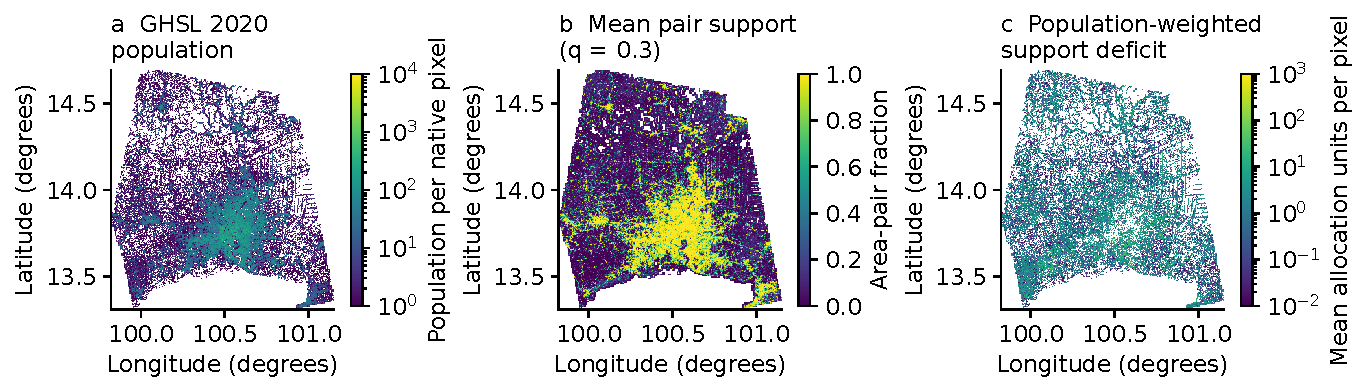
\includegraphics[width=\linewidth]{figures/F1_chao_spatial.pdf}
\refstepcounter{figure}\label{fig:spatial}
\end{figure}
\begin{table}[htbp]\centering
\caption{Native-model support deficits.}\label{tab:baseline}
\begin{tabular}{lrrrr}\toprule
Support rule & \shortstack{Population deficit\\(million units)} & \shortstack{Population\\deficit (\%)} & \shortstack{Built-surface deficit\\(km$^2$)} & \shortstack{Area\\deficit (\%)}\\\midrule
Valid unwrapped & 0.268 & 1.19 & 31.9 & 17.89 \\
Joint, $q=0.2$ & 1.665 & 7.40 & 197.5 & 57.44 \\
Joint, $q=0.3$ & 3.020 & 13.42 & 325.6 & 68.77 \\
Joint, $q=0.4$ & 4.891 & 21.74 & 464.6 & 76.83 \\
\bottomrule\end{tabular}

\end{table}

Unwrapped validity alone and the coherence-screened quantities are substantially different (Table~\ref{tab:baseline}). Raising $q$ from 0.2 to 0.4 changes the mean population deficit from \PopTwenty{} to \PopForty{} million. This range is a definition sensitivity, not a confidence interval. The weighted support curves retain information lost by applying one majority threshold to every coarse cell.

\begin{figure}[htbp]\centering
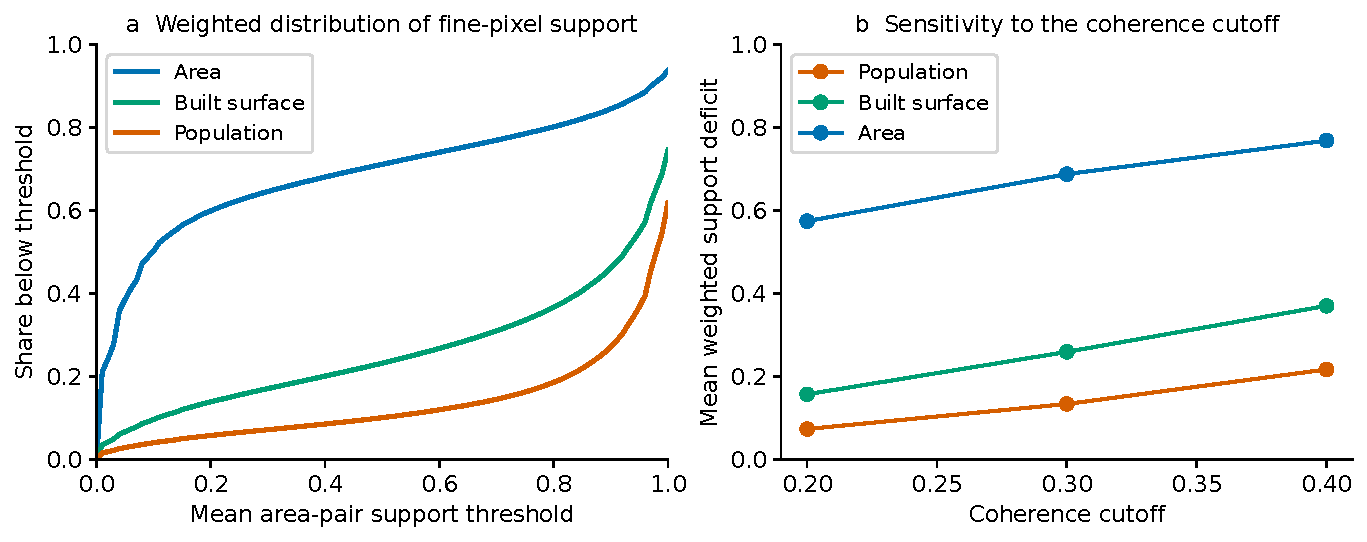
\includegraphics[width=\linewidth]{figures/F2_support_curves.pdf}
\refstepcounter{figure}\label{fig:curves}
\end{figure}

\subsection{Coarse uniform allocation increases the estimated support deficit}
With support, native population and AOI total held fixed, uniform allocation within 1-km cells yields \UniformOneMin{}--\UniformOneMax{} million mean population units in deficit, compared with the native-model reference of \PopThirty{} million. This is \UniformBiasMin{}--\UniformBiasMax{}\% higher across the four origins. Aggregate allocation discrepancy grows across the examined 250--2,000-m scales (Fig.~\ref{fig:scale}). The center approximation also changes with scale and origin; its variability cannot be interpreted as a measurement uncertainty distribution.

The signed discrepancy equals the integrated population--support covariance in Eq.~\ref{eq:covariance}. Positive aggregate covariance in this case means that uniform redistribution moves some population away from better-supported fine locations. Individual cells can have either sign, as the local discrepancy plot shows. The discrepancy depends on the within-cell association between population and support, as expressed by Eq.~\ref{eq:covariance}. Projection to a 25-m rather than 50-m integration grid changes the 1-km uniform population estimate by at most 0.00024 percentage points of the AOI total, far below the allocation differences being compared. A separate pixel-center grouping diagnostic across 250--2,000-m squares reproduces the covariance identity to numerical precision and satisfies its Cauchy--Schwarz bound; these scale-sensitivity values are not pooled with the direct-geometry estimates (Supplementary S8).

The 1-km effect persists when all boundary-crossing cells are excluded. Across four origins, the complete interior cells contain \InteriorPopulationMin{}--\InteriorPopulationMax{}\% of domain population, and uniform allocation exceeds their own native-model deficit by \InteriorBiasMin{}--\InteriorBiasMax{}\%. Interior cells account for \InteriorErrorMin{}--\InteriorErrorMax{}\% of the full-domain signed uniform-allocation difference. Thus boundary treatment does not explain the primary allocation effect. Supplementary S7 separates complete, partial and outside-center cells and reports both methods under each origin.


\begin{figure}[htbp]\centering
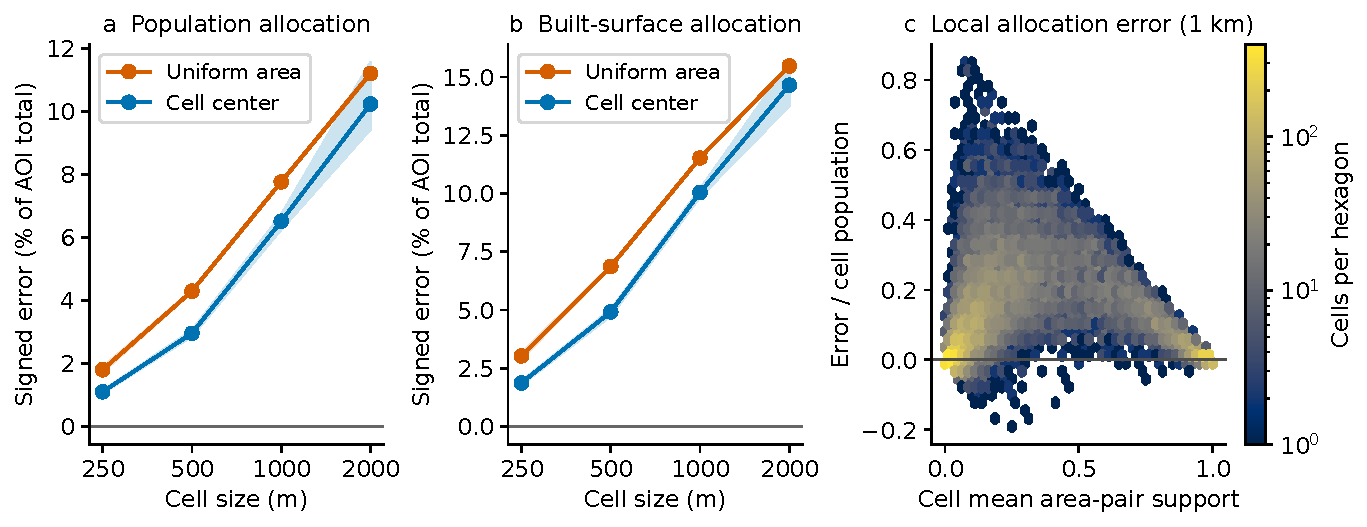
\includegraphics[width=\linewidth]{figures/F3_allocation_scale.pdf}
\refstepcounter{figure}\label{fig:scale}
\end{figure}

A user-selected discrepancy tolerance can be compared with the analytic scale/origin bound when the fine-scale inputs are available. Bounds above a tolerance remain inconclusive even when net differences are small (Supplementary S9).

\subsection{Sensitivity to pair sampling and population models}
The legacy 28-pair date graph contains 54 dates, 26 components and no independent cycles. It cannot stand in for a complete time-series inversion network. The 224-pair sampling graph is also not fully connected: it has 225 dates and 29 components. In contrast, the 2016--2022 catalogue graph has 288 dates and one component. Catalogue-level connectivity does not establish pixel-level validity.

The nested 28-, 56-, 112- and 224-pair means give population deficits of \SampleTwentyEight{}, \SampleFiftySix{}, \SampleOneTwelve{} and \SampleTwoTwentyFour{} million, respectively (Supplementary Fig.~S3). The nested 28-pair subset is selected from the expanded pool and differs from the original 28 pairs used in the primary 3.020-million calculation. Legacy leave-one-year-out results range from 2.820 to 3.181 million. Within the fixed 224-pair pool, the central 95\% range of the 100 stratified 28-pair draws is 2.665--4.072 million. That conditional sampling range is wider than the differences between several individual nested means and cannot be converted into a confidence interval for final product quality. Longer-baseline groups have larger mean deficits in both samples. Differences between sample sizes also reflect changes in baseline and seasonal composition.

Deleting each shared acquisition date changes the $q=0.3$ equal-quarter population deficit by $-0.386$ to $+0.165$ pp. These are dependent support sensitivities, with no velocity re-inversion or confidence interval (S20). Spatial rankings are more stable than the totals: across 539 eligible fixed geographic blocks, nested 28-, 56- and 112-pair deficit-amount ranks correlate 0.9940, 0.9992 and 0.9994 with the 224-pair comparator. Top-decile overlaps nevertheless change (Supplementary Fig.~S4). This is descriptive stability, not validation of a measurement-priority rule.

On pixels jointly valid in the four population/epoch layers, the $q=0.3$ deficit is \GHSLJointPct{}\% for native GHSL 2020 and \WPJointPct{}\% for WorldPop 2020. Joint coverage excludes \JointExcluded{} thousand GHSL population units from the full primary domain. Equalizing the two models to the same joint-domain total gives \GHSLJointCommon{} versus \WPJointCommon{} million mean deficit units, so total-population differences do not explain the discrepancy. At fixed 30-arc-second resolution, GHSL's 2015 and 2020 shares are \EpochOldPct{}\% and \EpochNewPct{}\%. These epoch sensitivities are smaller than the native-model contrast here, without establishing which model is accurate (Fig.~\ref{fig:population}).

\begin{figure}[htbp]\centering
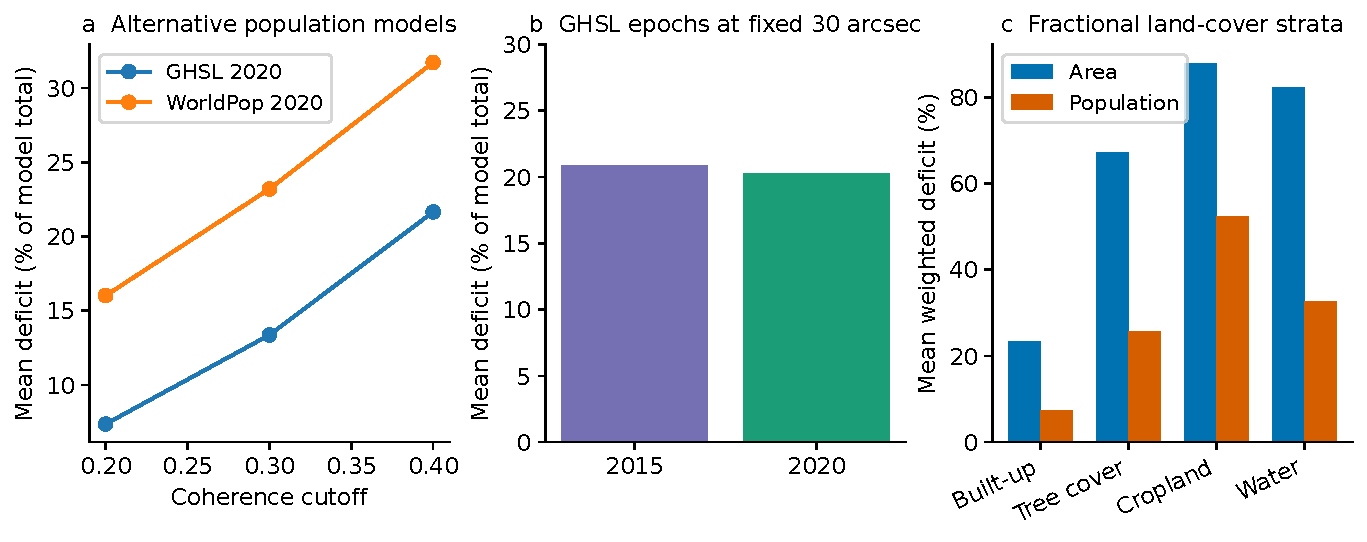
\includegraphics[width=\linewidth]{figures/F5_population_models.pdf}
\refstepcounter{figure}\label{fig:population}
\end{figure}

\paragraph{Crossing population model and pair selection.} On the fixed GHSL--WorldPop common domain, both models are normalized to 22.358 million population units. At 1 km, uniform allocation exceeds the native-model deficit by 55.38--55.64\% for GHSL with the legacy 28 pairs and 51.29--51.51\% with the expanded 224 pairs. The corresponding WorldPop differences are 9.03--9.07\% and 8.64--8.68\%. All 16 model--sample--origin combinations have positive differences; normalized by the common total, these span 7.40--7.53 percentage points for GHSL and 2.09--2.13 for WorldPop. The direction therefore persists across these inputs, while its magnitude is strongly population-model dependent. The original approximately 58\% difference is specific to its full-domain GHSL case. Changing 28 to 224 pairs changes selection and composition as well as sample size; the comparison is not an isolated sample-size effect. Supplementary S18 reports every origin and the numerical convergence check.


The Fresno population comparisons separate source totals from spatial allocation. Against 2020 Census blocks, total-normalized 1-km GHSL and WorldPop allocations have weighted absolute percentage error (WAPE; summed absolute unit discrepancies divided by the Census total) of 57--59\%, below an area-only baseline (S24). A 100-m comparison normalizes GHSL and the California population surface (CA-POP) to the same Census block counts; the outside-footprint allocation differs by 0.143 pp, with mixed tract-level directions (S25). CA-POP uses the same Census counts as inputs, so this is an allocation sensitivity.

The American Community Survey (ACS) 2017--2021 benchmark uses 319 complete Fresno block groups. Their areas are not uniformly larger than the 1-km source pixels: 80.25\% are below 1 km$^2$. Source-cell uniformity therefore remains material. The ACS total is 493,571; Census P1 differs by $-0.36\%$, GHSL by $+10.57\%$ and WorldPop by $+6.03\%$. The aggregate Census total falls within the ACS 90\% margin of error, but this agreement does not validate household locations (S26). Spatially held-out total recalibration gives GHSL WAPE 33.24--33.85\% versus 33.16\% in sample, and WorldPop 32.34--32.98\% versus 32.29\% (S20). These block-group results use a different domain and aggregation from the block-level comparison; they do not measure improved fine-scale accuracy.

Municipal residential eligibility gives a further allocation constraint, with substantial missing classification. Strict eligibility contains 85.22\% of mapped GHSL allocation and 89.30\% of mapped CA-POP allocation, while 32.22\% and 31.26\% of complete allocation are unmapped. On the restricted common domain, the deficit falls from 0.0927\% to 0.0508\% for GHSL and from 0.0572\% to 0.0414\% for CA-POP. That domain covers 89.13\% of complete Census population, below the exploratory 90\% reporting gate; it supports only a limited-domain sensitivity (S27).

\subsection{Estimation error and availability under controlled missingness}
For random and spatial masks unrelated to density, aggregate mean bias is small across repetitions, while the center method has larger sample-to-sample variation. Density-associated masking changes the sign and size of the error (Fig.~\ref{fig:masking}). At 30\% removal and 10-pixel cells with zero origin, uniform allocation underestimates the known removed population by 14.17\% when high-density locations are preferentially removed and overestimates it by 120.35\% when low-density locations are preferentially removed. Large relative errors occur when the removed population is small. We also report errors normalized by the total test-domain population.

Built-area weights reduce error in these GHSL-based scenarios but retain nonzero errors and shared-input dependence. The synthetic hazard experiments additionally show that support deficit alone does not identify threshold-exposed population: the unknown allocation can contain very different hazard shares under the three constructed velocity fields. The conservative identification interval contains the known truth by construction; its width expresses missing information rather than recovered motion. Fresno masking outputs repeat the same protocol and are supplied in the Supplementary Information.

Structured masks leave substantial allocation unestimated even when errors on computable units are small. At 30\% removal, 10-pixel units and a $-5$ mm yr$^{-1}$ cutoff, prevalence leaves less than 0.0001\% of the original allocation unestimated under random masks, versus 11.35\%, 18.16\% and 28.66\% under clusters, high-spread removal and low-spread removal. All rules are compared on their common-computable domain. Prevalence has smaller mean local L1 error than median classification in the first three mechanisms; the median rule has smaller L1 under low-spread removal. Under high-spread removal, the common-domain mean signed errors are positive: +0.0884 pp for prevalence and +0.1034 pp for the median rule. Whole-domain bound widths remain 24.12--34.90 pp across these mechanisms (S12, S14).

These rules estimate the hidden fine-pixel class allocation. This target differs from assigning a whole Census block to its median-rate class. The irregular-block experiment makes that distinction visible even before masking: at $-5$ mm yr$^{-1}$, median classification has 0.01167 pp local L1 discrepancy against the fine-allocation target. After 30\% removal, prevalence leaves 0.20\% unestimated under random pixels, versus 23.01\% under one contiguous hole and 28.64\% under four holes; the median rule leaves 9.41\%, 26.80\% and 32.61\%. Mean whole-domain bound widths are 30.02, 24.02 and 30.97 pp. Small errors on computable blocks do not identify class allocation under the gaps (S15).

For the actual LiCSBAS final mask, a worst-case finite-domain calculation bounds the share of allocation in each LOS threshold class without assigning a physical rate to unsupported pixels. Unsupported allocation accounts for 0.2944 percentage points of the fixed domain, so the identification interval has that width at each of the $-2$, $-5$ and $-10$ mm yr$^{-1}$ thresholds. This finite bound is small in population-share terms but leaves the motion in unsupported locations unknown (Supplementary S13).


\begin{figure}[htbp]\centering
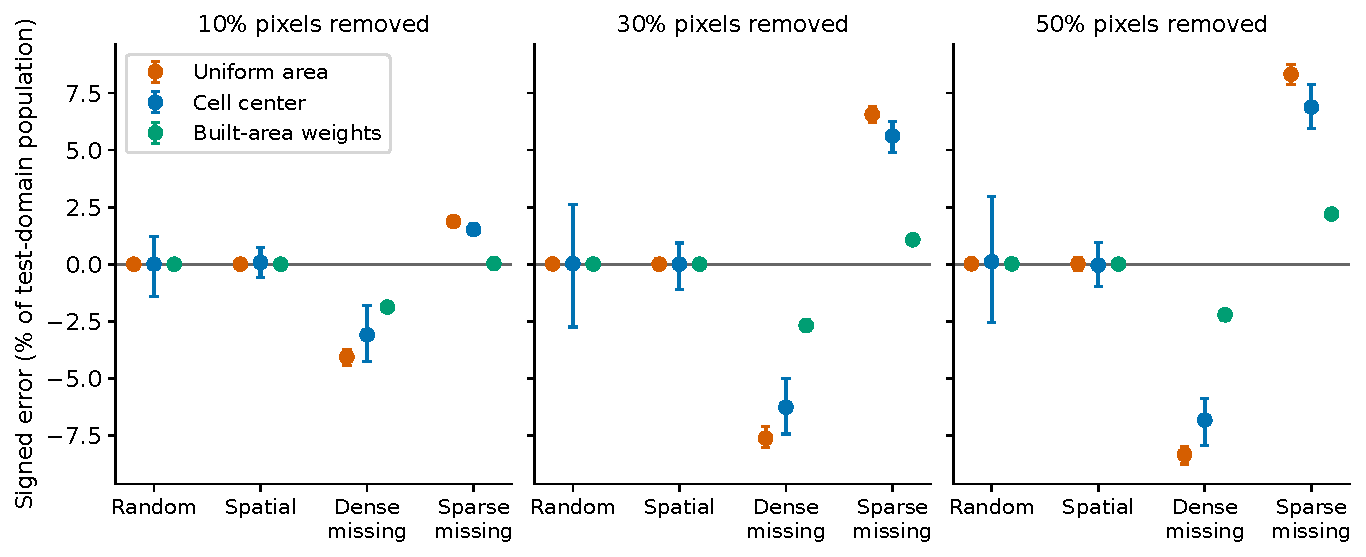
\includegraphics[width=\linewidth]{figures/F4_masking.pdf}
\refstepcounter{figure}\label{fig:masking}
\end{figure}

\subsection{Input support, final quality and internal residuals}
Full-stack quality rejection leaves 431 of 437 pairs for inversion; the training branch retains 382 of 393 inputs. The full quality mask accepts 97.02\% of pixels and 99.71\% of the small area's allocated population. Among pixels with matched-input mean support below 0.2, 83.34\% still pass the fixed multi-index mask; the 0.8--1 group has 99.72\% acceptance. Low coherence-screened support is therefore not equivalent to final processing rejection (Fig.~\ref{fig:matched}). Neither acceptance nor rejection is independent physical truth.

At a legacy-support threshold of 0.5, the low-support/accepted and high-support/rejected categories contain 208,609 and 30,637 population allocation units, respectively. That legacy comparison also changes the acquisition period and sample. The matched-input bins provide the within-period comparison: median bootstrap velocity spread is 1.343 versus 1.185 mm yr$^{-1}$ and median inversion residual is 0.673 versus 0.368 mm for the lowest and highest support groups. These associations describe quality differences rather than a binary validity surrogate.

All 44 held-out edges met the prediction and reference requirements. Pooled held-out LOS displacement root-mean-square error (RMSE) is 0.984 mm across evaluable observations. Training-mask accepted and rejected locations give 0.699 and 5.150 mm, respectively; the lowest and highest training-support bins give 2.338 and 0.412 mm. On common evaluable observations, time-series differences, training linear velocity and a zero-displacement baseline give 0.984, 11.751 and 11.784 mm. The held-out pairs connect dates already represented in training. Shared acquisition dates and atmospheric phase limit these residuals to internal reconstruction; they do not measure independent velocity accuracy. Exclusions and per-pair results are retained in Supplementary S17.

We additionally compare the same GHSL population field against two distinct support summaries on this processing grid: mean support across the 437 full-stack input pairs and the final LiCSBAS full-stack quality mask. Direct intersections between the native source cells and 1-km UTM cells show that uniform-area allocation increases the mean deficit by 3.066--3.189 percentage points of the fixed AOI population for the 437-pair support field, but by 0.108--0.117 points for the final quality mask across four grid origins. Their native deficits are 3.4539\% and 0.2944\%, respectively. These support definitions carry different processing information; their contrast is not an error comparison, and neither identifies deformation in invalid pixels. The source-to-grid intersections and numerical checks are reported in Supplementary S19.

\begin{figure}[htbp]\centering
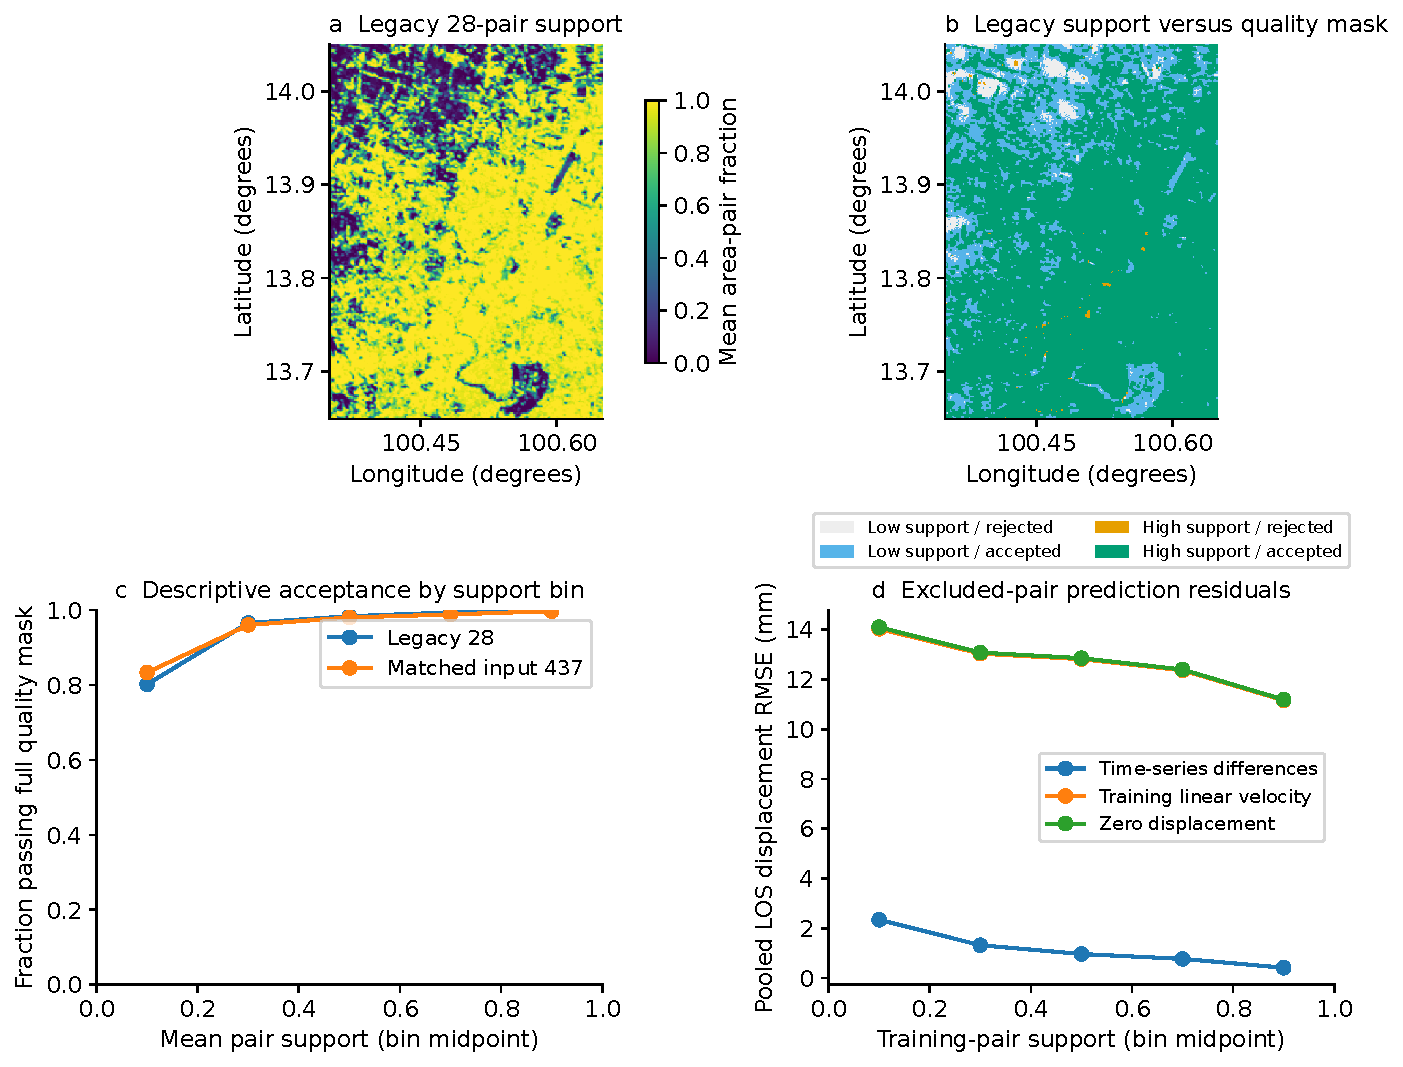
\includegraphics[width=\linewidth]{figures/F7_matched_processing.pdf}
\refstepcounter{figure}\label{fig:matched}
\end{figure}
Training-only filtering exposes a coverage--residual tradeoff. Raising coherence from 0.2 to 0.4 reduces accepted population allocation from 99.40\% to 95.34\%, while pooled excluded-edge displacement RMSE falls from 0.491 to 0.388 mm; population-weighted RMSE changes from 0.344 to 0.336 mm. At 0.7, only 41.04\% remains. Other quality metrics show nonmonotonic error responses; results for all 18 rules are reported in S21. These are post-filters on a fixed inversion, not estimates of absolute velocity accuracy (S21).

\subsection{Transfer across support definitions and regions}
In Fresno, the DWR observation-cell union covers 78.49\% of the 495.51-km$^2$ rectangle but contains \DWRSupportPct{}\% of its GHSL allocation. Of \DWRTotal{} allocation units, \DWRUnsupported{} fall outside the footprint. At 1 km, uniform allocation gives \DWRUniformMin{}--\DWRUniformMax{} outside-support units, an additional 1.2--1.3 pp of the AOI total. Its large relative multiplier therefore has a small baseline. Center sampling also varies with grid origin (Fig.~\ref{fig:dwr}).

On the complete Census-block domain, the Census-population-weighted DWR area-coverage share is 99.19\%, versus 99.74\% for native GHSL allocation (S23). This normalized-share contrast reflects relative spatial weights, whereas the 12.20\% GHSL--Census total difference is a separate diagnostic. Multiplying all weights by one constant leaves either share unchanged.

The separate DWR rate example assigns Census block counts to the median observed vertical-rate class, following the published workflow. After annualizing each exact time window, the six-window 2015--2021 median covers blocks containing 95.70\% of complete-block Census population; 64.99\% of covered population falls below $-5$ mm yr$^{-1}$. Annual windows and the cumulative endpoint rate yield different classes. This interpolated vertical-rate transfer is distinct from the Bangkok LOS field and provides no independent validation of it (S28).

\begin{figure}[htbp]\centering
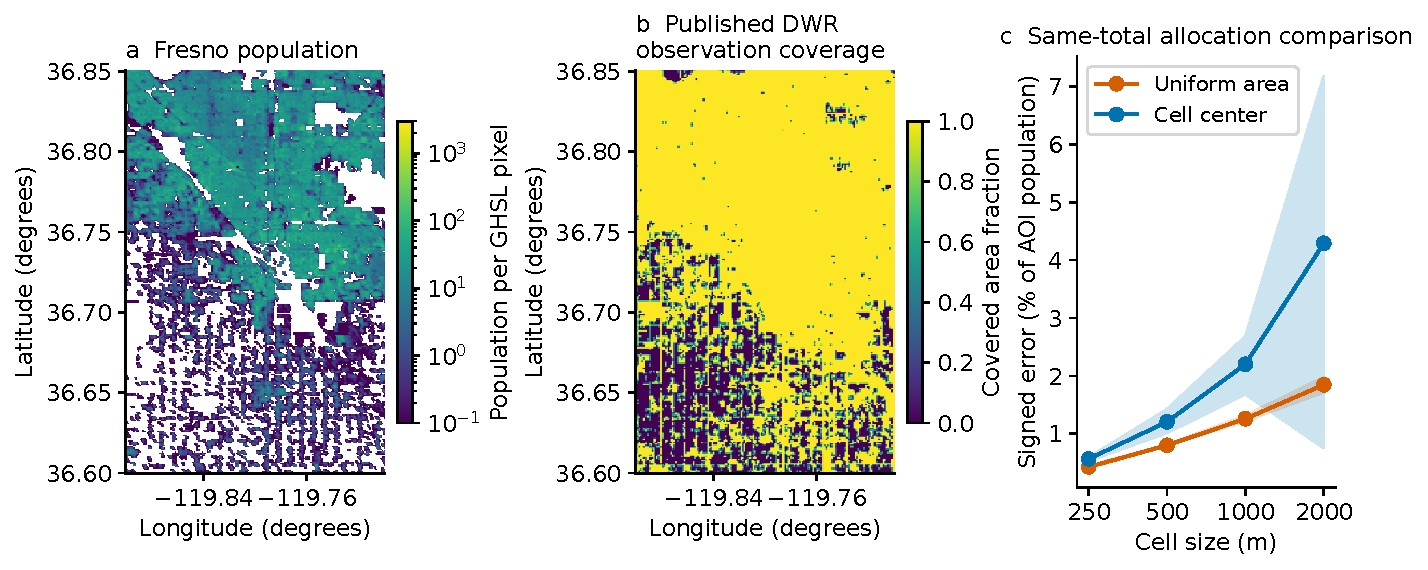
\includegraphics[width=\linewidth]{figures/F6_dwr.pdf}
\refstepcounter{figure}\label{fig:dwr}
\end{figure}

Across 96 fixed-region scale/origin/cutoff designs, uniform-minus-native differences are only 0.026--0.186 pp in Los Angeles and 0.051--0.372 pp in Davis--Sacramento. The positive direction transfers, but these small effects do not generalize the approximately 58\% primary relative difference (S29).

External GNSS agreement is mixed. Native-pixel RMSE in Los Angeles is 14.49 mm yr$^{-1}$ under provider reference P597 and 1.30 under location-selected local control MHMS (11 validation stations). Davis--Sacramento gives 8.94 under P266 and 10.85 under UCD1 (four stations). Controls are excluded from validation; every sampling radius and both frames are retained. Archived source-version conflicts, temporal-model differences and station dependence limit interpretation. These results cannot be transferred to our Bangkok inversion (S30).

\FloatBarrier
\section{Discussion}
\subsection{The aggregation effect and its dependence on inputs}
The matched-input comparisons establish a material change in population-weighted support summaries when fine spatial allocation is replaced by uniform coarse allocation. The effect persists in complete interior cells, so boundary handling does not explain the primary result. Crossing population models and pair selections gives a consistent positive direction across the 16 tested cases, but the relative difference is much smaller with WorldPop than with GHSL. The approximately 58\% difference is specific to the primary GHSL case; the crossed comparisons show how the magnitude changes with the population distribution. It does not establish a universal correction factor.

\subsection{Mechanism and choice of allocation method}
The mechanism is the loss of the population--support cross moment when a coarse mean support is multiplied by a coarse population total. Its signed effect follows within-cell covariance, explaining both the primary aggregate overestimation and the opposite directions under density-associated masking. Small aggregate biases under density-independent masks also identify conditions in which uniform allocation can be adequate. A finer overlay is useful when the selected population model's spatial structure is appropriate to retain; agreement with that reference does not establish household-level accuracy.

Method choice follows the available information. A complete-case overlay describes allocation inside its observed domain. A center rule is inexpensive but can miss subcell structure and boundary coverage. Uniform-area transfer is appropriate when its uniformity approximation produces acceptably small error for the intended summary. Building weights add ancillary assumptions and can share inputs with the population model. Imputation, multiple sensors and ground measurements add information about deformation and require their own evaluation. Our experiments quantify the effects of support accounting choices that accompany such measurements.

\subsection{Applicability and evidence limits}
The principal Chao Phraya statistic averages over area and selected interferometric pairs. It cannot identify how many unique residents lacked all observations, nor whether a final product is valid at their locations. A coherence pass is insufficient for a reliable velocity, and a failed pass does not prove permanent radar blindness. The matched processing experiment adds evidence about one specified processing chain: sampled support and its final quality mask are distinct, while held-out edge residuals assess internal reconstruction. Shared acquisition dates and atmospheric signals limit the physical interpretation of those residuals.

The crossed comparison and separate common-coverage population summaries both show that population-model choice is consequential. Local census geography, building occupancy and rapidly changing settlements are not measured by this overlay. The primary domains, added California rectangles and deliberate sampling designs do not establish a worldwide error magnitude. The primary domain inherits the finite source-VLM footprint; conclusions do not extend to locations outside it. LiCSAR's sampled pair support and DWR's published observation footprint remain different support objects, even though the same mass-preserving accounting protocol can be applied to both.

\paragraph{Validation scope and limitations.} Controlled masks and geometry/conservation checks evaluate numerical accounting against declared references. LiCSBAS excluded-edge residuals evaluate internal reconstruction, while the published DWR footprint and rate examples test transfer across product definitions. Census/CA-POP comparisons assess population-model allocation at reporting-unit scale, and ACS supplies a survey-based aggregate agreement benchmark with replicate-based uncertainty. These sources do not establish household locations or deformation in permanently unsupported pixels. The added California comparison supplies archived independent GNSS observations for an external LOS product, with mixed results and a temporal-model limitation; it does not validate our Bangkok inversion. No matched independent GNSS or leveling validation has been obtained for that inversion.



\paragraph{Earlier estimates and source attribution.} The submitted 3.772492-million center-majority total is reproducible, but it is not a verified count of people exposed to subsidence in missing areas. The earlier center-majority statistic differs from the mean support deficit defined here; their relationship and input provenance are documented in Supplementary S2. We have removed the exploratory Iran branch from quantitative applications. Its archived rate and mask correspond to the 2014--2020 product associated with Haghshenas Haghighi and Motagh (2024). No Iran result or new/old Iranian product comparison contributes to the quantitative conclusions. Supplementary S3 documents the attribution correction and distinguishes the newer products of Payne et al.\ \citep{haghshenas2024iran,payne2025iran,payne2024data}.

\section{Conclusions}
Spatial aggregation changes population-weighted InSAR support summaries by omitting the within-cell population--support cross moment. Fixed-input and complete-interior comparisons establish this effect. Its direction persists across the tested population models and pair selections, while its magnitude depends on the inputs and study area. Controlled missingness identifies conditions under which the error reverses, aggregate bias is small or substantial allocation remains unestimated. The published-support and regional comparisons show that transfer also depends on the support definition; external GNSS agreement differs between regions. Population-weighted reporting should therefore specify its domain and support field, preserve extensive quantities and their cross moments, and report sensitivity to allocation and sampling. Deformation in unsupported locations remains unknown.

\section*{Data Availability}
Public input data are obtained from COMET LiCSAR, GHSL, WorldPop, ESA WorldCover, the U.S. Census Bureau, California DWR, the archived ARIA California products, NGL and City of Fresno municipal GIS. Exact source-product identifiers, acquisition methods and input checksums are documented in the Supplementary Information and accompanying reproducibility materials. Source-provider terms govern access to and reuse of third-party inputs. Frozen processed analysis inputs, full reference and replicate tables, figure source data and the manuscript number ledger are publicly available with the versioned scientific reproduction package.

\section*{Code Availability}
The scientific reproduction package is publicly available at the fixed GitHub release \href{https://github.com/niubisile-wq/openinsar-observability-bias/releases/tag/v0.6.0}{v0.6.0}. It contains the experiment code, configurations, input manifests and checksums, processed analysis inputs, full reference outputs, environment records and reviewer reproduction instructions. Companion assets supply portable inputs and selected complete source products for S15, S20--S21, S27, S29--S30, with file-level checksums. The complete ACS files and official Census source archives used in S25 remain available at v0.4.1. The reviewer guide provides reproduction and numerical-comparison commands for the processed inputs and reference outputs in release v0.6.0. Other provider-controlled original products and the complete interferogram processing stacks are obtained separately through the documented acquisition routes. The earlier DOI \href{https://doi.org/10.5281/zenodo.21444768}{10.5281/zenodo.21444768} archives v0.3.0; a revised DOI deposit remains pending.
\def\bibfont{\small}
\bibliography{references}
\section*{Author Contributions}
Z.L.: analysis and manuscript preparation. W.X.: supervision and manuscript revision.
\section*{Additional Information}
\subsection*{Competing interests}
The authors declare no competing interests.
\section*{Figure legends}

\noindent\textbf{Figure~\ref{fig:spatial}.} Fixed-footprint Chao Phraya analysis: GHSL 2020 population, mean joint area--pair support at $q=0.3$, and their allocation-weighted support deficit. Maps use the native GHSL grid; logarithmic population displays leave zero values blank. Panels show population allocation and observation support.

\noindent\textbf{Figure~\ref{fig:curves}.} Continuous support summaries. Left: weighted distributions of native-pixel mean support for $q=0.3$. Right: mean deficits under three coherence cutoffs. All curves use the same geographic domain, independent of velocity-threshold selection.

\noindent\textbf{Figure~\ref{fig:scale}.} Same-input allocation discrepancies at $q=0.3$. Lines are means across four origins and bands span those origins, not confidence intervals. Errors are normalized by fixed AOI exposure totals. The local 1-km plot shows uniform-minus-native discrepancy divided by each nonzero cell population; its negative values demonstrate that aggregate overestimation is not universal at the cell scale.

\noindent\textbf{Figure~\ref{fig:population}.} Population and land-cover sensitivities. Population models and epoch comparisons use their common valid domain; the epoch panel holds spatial resolution fixed. Fractional land-cover summaries use the primary geographic domain and preserve the within-GHSL-pixel allocation assumption. WorldCover 2021 v200: \copyright{} ESA WorldCover project 2021; contains modified Copernicus Sentinel data (2021) processed by the ESA WorldCover consortium.

\noindent\textbf{Figure~\ref{fig:masking}.} Artificial missingness in the fixed Bangkok rectangle, using 10-fine-pixel coarse cells and zero origin. Symbols show mean signed error and bars the 2.5th--97.5th percentiles of 100 introduced-mask repetitions. The denominator is the entire test-domain population, enabling comparison when the removed population is very small. Complete relative-error, local-error, scale and origin results are provided separately.

\noindent\textbf{Figure~\ref{fig:matched}.} Matched LiCSBAS experiment in the fixed Bangkok rectangle. The legacy support map uses the 2016--2022 sample; its high/low split is 0.5 in panel b, compared with the 2019--2020 full-stack quality mask. Panel c separately includes the matched 437-pair input diagnostic. Both diagnostics use coherence cutoff $q=0.3$. Panel d groups held-out prediction residuals using training pairs only. Lines connect the support-bin summaries.

\noindent\textbf{Figure~\ref{fig:dwr}.} Second-region accounting using actual DWR observation-cell polygons in a fixed Fresno rectangle. Polygon intersections are unioned before assigning population. The deficit reference is small because the observed footprint covers almost all allocated population despite leaving appreciable area uncovered. Scale-comparison errors use the full AOI population as denominator; bands span four origins.

\section*{Table legend}
\noindent\textbf{Table~\ref{tab:baseline}.} Native-model support deficits in the primary geographic domain and legacy 28-pair sample. Each percentage uses its stated population or area denominator.
\end{document}
